\documentclass[aspectratio=169,9pt]{beamer}
\usetheme[progressbar=frametitle,numbering=fraction,block=fill,sectionpage=none]{metropolis}
\usepackage[T1]{fontenc}
\usepackage{amsmath,amssymb}
\usepackage{booktabs}
\usepackage{tikz}
\usetikzlibrary{arrows.meta,positioning,calc}
\usepackage{graphicx}
\graphicspath{{../results/}{../results/live_2026_10/}}
\setbeamerfont{frametitle}{size=\large}
\setbeamerfont{caption}{size=\scriptsize}
\setbeamertemplate{caption}{\insertcaption}
\definecolor{ink}{HTML}{0b0b0b}
\definecolor{muted}{HTML}{52514e}
\definecolor{blue}{HTML}{2a78d6}
\definecolor{orange}{HTML}{eb6834}
\definecolor{aqua}{HTML}{1baf7a}
\definecolor{red}{HTML}{e34948}
\definecolor{grey}{HTML}{9a9890}
\setbeamercolor{progress bar}{fg=blue}
\setbeamercolor{alerted text}{fg=orange}
\setbeamercolor{frametitle}{bg=ink,fg=white}
\newcommand{\Fanon}{\mathcal{F}^{\mathrm{anon}}}
\newcommand{\Fid}{\mathcal{F}^{\mathrm{id}}}
\newcommand{\For}{\mathcal{F}^{\mathrm{oracle}}}
\newcommand{\LBR}{L_{\mathrm{BR}}}
\newcommand{\takeaway}[1]{\vspace{2pt}\begin{beamercolorbox}[rounded=true,sep=4pt]{block body}\small\textbf{#1}\end{beamercolorbox}}

\title{Rent or Toxicity?}
\subtitle{Strategic exploitability of learning market makers with public wallet information}
\author{Deepu Pradeep \quad Miguel Betran Menz}
\institute{6.S974 Games, Learning, and Security --- Workshop 1\\ Example 4: an algorithmic market with adaptive agents}
\date{October 27, 2026}

\begin{document}
\maketitle

% ============================================================ (a) motivation
\section{Motivation and question}

\begin{frame}{The system: a market where everyone can see who is trading}
\begin{columns}[T]
\begin{column}{0.55\textwidth}
\textbf{Hyperliquid}, an on-chain exchange
\begin{itemize}
\item \textbf{Makers} post standing offers to buy and sell (a \emph{quote}); \textbf{takers} accept them (a \emph{fill}). The public record of fills is the \emph{tape}.
\item Every order and both sides of every fill carry a \textbf{public wallet address}.
\item Prices live on a coarse grid (one step $=$ a \emph{tick}); same-price orders are served first-in-first-out.
\item Takers are \textbf{informed} (trade only when the maker will lose) or \textbf{uninformed}. Flow with many informed takers is \emph{toxic}.
\end{itemize}
\end{column}
\begin{column}{0.45\textwidth}
\textbf{The puzzle}
\begin{itemize}
\item Independent learning makers settle on quotes \emph{wider} than the competitive one, without communicating: a \textbf{rent} (tacit collusion).
\item But a wide quote is also the correct charge for toxic flow.
\item On the tape, \textbf{rent and toxicity look identical.}
\end{itemize}
\vspace{2pt}
\textbf{Three players, three decisions}\\[1pt]
{\small the \emph{incumbents}: how wide; whether to stay in the queue \\ an \emph{entrant}: which quotes to undercut, which fills to take \\ the \emph{venue}: public identities? tick size? pay for position?}
\end{column}
\end{columns}
\end{frame}

\begin{frame}{What we want to learn}
\begin{enumerate}
\item[\textbf{RQ1}] \textbf{What is public wallet identity worth} to an entrant, beyond the anonymous tape --- and through which mechanism?
\item[\textbf{RQ2}] \textbf{How exploitable is a learned cartel's rent?} How much can an adversary take or destroy, and does more rent mean more vulnerability?
\item[\textbf{RQ3}] \textbf{When the grid pins the quote at one tick}, where does rent live, and which venue and maker levers decide who holds the toxic flow?
\end{enumerate}
\vspace{6pt}
\textbf{Why it is a game.} The entrant's weapon --- undercutting, or taking only the benign fills --- is exactly what the makers' learned \emph{reaction function} is tuned to punish; and the venue decides what each side is allowed to know.
\vspace{6pt}
\takeaway{Headlines today: the rent is fully exploitable by an entrant that solves the cartel's reaction function; identity's value is a lag story; and on the real book the makers who earn the spread are the ones avoiding the toxic wallets.}
\end{frame}

% ============================================================ (b) model
\section{Mathematical model}

\begin{frame}{One period of the game}
\centering
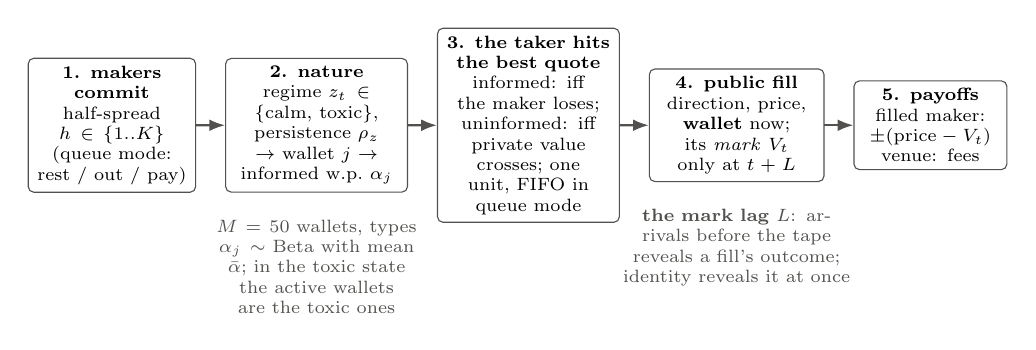
\begin{tikzpicture}[x=1cm,y=1cm,scale=0.92,transform shape,
  box/.style={draw=muted,rounded corners=2pt,fill=white,align=center,font=\scriptsize,minimum height=0.9cm,inner sep=3pt},
  arr/.style={-{Latex[length=2mm]},thick,color=muted},
  lab/.style={font=\scriptsize,color=muted,align=center}]
\node[box,text width=2.1cm] (q) at (0,0) {\textbf{1. makers commit}\\ half-spread $h\in\{1..K\}$ \\ (queue mode: rest / out / pay)};
\node[box,text width=2.3cm,right=0.4cm of q] (n) {\textbf{2. nature}\\ regime $z_t\in\{$calm, toxic$\}$, persistence $\rho_z$ \\ $\to$ wallet $j$ $\to$ informed w.p.\ $\alpha_j$};
\node[box,text width=2.3cm,right=0.4cm of n] (f) {\textbf{3. the taker hits the best quote}\\ informed: iff the maker loses; uninformed: iff private value crosses; one unit, FIFO in queue mode};
\node[box,text width=2.2cm,right=0.4cm of f] (p) {\textbf{4. public fill}\\ direction, price, \textbf{wallet} now; \\ its \emph{mark} $V_t$ only at $t+L$};
\node[box,text width=1.9cm,right=0.4cm of p] (r) {\textbf{5. payoffs}\\ filled maker: $\pm(\text{price}-V_t)$ \\ venue: fees};
\draw[arr] (q) -- (n); \draw[arr] (n) -- (f); \draw[arr] (f) -- (p); \draw[arr] (p) -- (r);
\node[lab,text width=3.2cm,below=0.25cm of n.south] {$M=50$ wallets, types $\alpha_j\sim$ Beta with mean $\bar\alpha$; in the toxic state the active wallets are the toxic ones};
\node[lab,text width=3.4cm,below=0.25cm of p.south] {\textbf{the mark lag} $L$: arrivals before the tape reveals a fill's outcome; identity reveals it at once};
\end{tikzpicture}
\vspace{2pt}
\begin{columns}[T]
\begin{column}{0.5\textwidth}\small
\textbf{Who decides what, with what information}
\begin{itemize}\setlength\itemsep{1pt}
\item \textbf{Incumbents} ($N=2,3$): tabular Q-learners, state $=$ (own last $h$, best rival's last $h$); identity-blind by construction. $2\times10^4$ training episodes, then \emph{frozen}.
\item \textbf{Entrant}: information set is a treatment, $\Fanon$ (tape) $\subset\Fid$ ($+$ wallets) $\subset\For$ ($+$ regime); a Bayesian filter gives $\alpha_{\text{next}}$.
\item \textbf{Venue}: identities public or not; tick; priority fee $f$.
\end{itemize}
\end{column}
\begin{column}{0.5\textwidth}\small
\textbf{Horizon and payoffs}
\begin{itemize}\setlength\itemsep{1pt}
\item $T=100$ periods per episode; regime chain and wallets persist across episodes.
\item Market-wide expected payoff of a best quote $h$ against informed share $\alpha$, closed form:
$\Pi(h;\alpha)=(1-\alpha)\,2x\bar\Phi(x/\sigma_L)-\alpha\mu e^{-x/\mu}$, $x=h\theta$
\item General-sum: the \emph{defenders' loss} is the statistic, not the attacker's gain.
\end{itemize}
\end{column}
\end{columns}
\end{frame}

\begin{frame}{Benchmarks are closed-form, so ``rent'' is measured, not estimated}
\begin{columns}[T]
\begin{column}{0.52\textwidth}\small
\begin{itemize}\setlength\itemsep{3pt}
\item $h^C=\min\{h:\Pi\ge0\}$: the \textbf{Nash} (competitive, break-even) quote --- any wider quote is profitably undercut.
\item $h^M=\arg\max_h\Pi$: the \textbf{joint-monopoly} quote.
\item $\bar\alpha=0.1,0.3,0.5$: $(h^C,h^M)=(2,13),(4,14),(8,17)$; the monopoly rent $\Pi^M-\Pi^C=1.90,1.38,0.66$.
\item \textbf{Rent index} $C=\dfrac{\Pi_{\text{nominal}}-\Pi^C}{\Pi^M-\Pi^C}\in[0,1]$: where a frozen cartel sits between Nash (0) and monopoly (1).
\item With adversary $A$: \textbf{best-response loss} $\LBR^A=\Pi_{\text{nominal}}-J(A)$; \textbf{fraction of rent destroyed} $\kappa_A=\LBR/(\Pi_{\text{nominal}}-\Pi^C)$. ``Rent units'' $=$ divided by $\Pi^M-\Pi^C$.
\end{itemize}
\end{column}
\begin{column}{0.48\textwidth}\small
\textbf{A worked example} ($\bar\alpha=0.3$, tick $0.5$)
\begin{itemize}\setlength\itemsep{2pt}
\item Two incumbents at $h=14$ split $\Pi(14)=1.50$.
\item An entrant at $13$ takes every fill: earns $\Pi(13)=1.49$; incumbents earn 0.
\item They answer at $12$; the entrant at $11$ earns $1.39$ \ldots\ the chase ends at $h^C=4$, $\Pi=0.12$.
\item \textbf{A learned cartel is a reaction function that does \emph{not} chase every time.} That restraint is the rent --- and the attack surface.
\end{itemize}
\vspace{4pt}
\textbf{Queue mode} (the one-tick book): spread pinned at $h$; actions \textsc{rest} / \textsc{out} / \textsc{rest-and-pay}; FIFO. All value is in \emph{which fills you take}: at $h^C$ a fill is worth $+1.10$ in the calm state, $-2.26$ in the toxic one.
\end{column}
\end{columns}
\end{frame}

% ============================================================ (c) prototype and evidence
\section{Prototype and evidence}

\begin{frame}[fragile]{The prototype, in one command}
\begin{columns}[T]
\begin{column}{0.47\textwidth}\small
\texttt{python experiments/demo.py} \quad (seconds)
\begin{enumerate}\setlength\itemsep{1pt}
\item prints the benchmarks: $h^C=4$, $h^M=14$, $\Pi(h)$
\item plays the shipped two-maker cartel alone: $C=0.86$
\item enters three adversaries under common random numbers
\item traces the exact best response, period by period
\end{enumerate}
\vspace{4pt}
\textbf{Package} (\texttt{github.com/pradeepu191/wargame}, 59 tests): \texttt{sim/} environment, learners, entrants, queue mode, benchmarks; \texttt{experiments/} every result below; \texttt{analysis/} the Hyperliquid pipeline (recorder, scoring, identity selection); \texttt{results/REPLICATION\_NOTES.md} logs each result with its command.
\end{column}
\begin{column}{0.53\textwidth}
{\tiny\begin{verbatim}
Entry (200 episodes each, same random numbers):
  adversary                     cartel loses  entrant earns  kappa_A
  undercut (one tick inside)            0.41           0.33     0.48
  markout (undercut if rent inferred)   0.47           0.41     0.55
  exact best response                   0.94           1.09     1.10

Trace: exact best response vs the cartel (quotes in ticks)
   t  inc0  inc1  entrant   taker         filled   payoff
   0    15    24       12   noise    buy  entrant   +1.21
   1    23    16       13   noise    buy  entrant   +7.86
   2    20    14       13   no trade
   5    21    19       14   informed buy  entrant   -5.77
   7    18    23       14   noise    buy  entrant  +11.79
\end{verbatim}}
\vspace{-4pt}
{\scriptsize The incumbents answer each entrant quote with their learned reaction; the entrant sits one tick inside what they are \emph{about to} quote and holds them where they never trained.}
\end{column}
\end{columns}
\end{frame}

\begin{frame}{Evidence 1 --- learners coordinate above the Nash point}
\centering
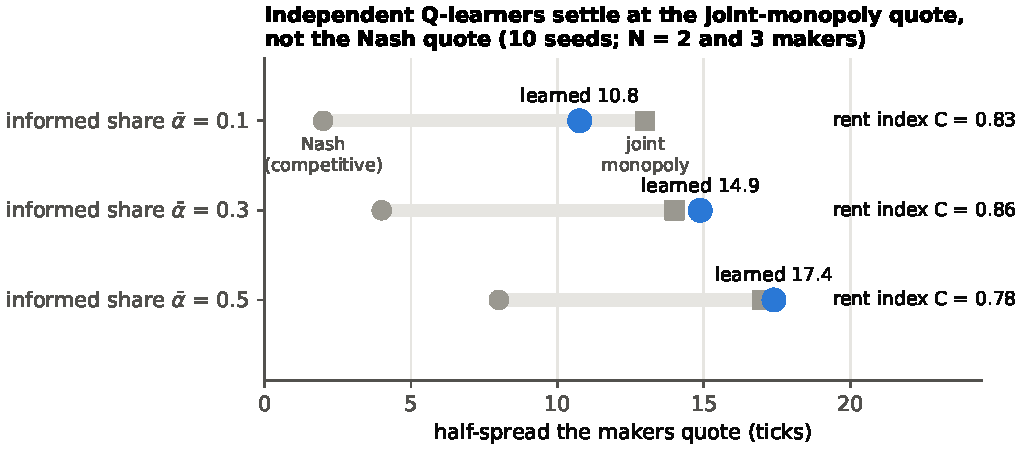
\includegraphics[width=0.7\textwidth]{fig_rent.pdf}
\vspace{2pt}
\begin{itemize}\small
\item Replicates Colliard--Foucault--Lovo; $C=0.71$--$0.87$ in every cell of a grid over $N$, learning rate, initialisation.
\item Mechanism is \textbf{restraint}: in 55--83\% of visited states undercutting would pay this period; in 96--100\% of those the learner forgoes it. Fills rotate; an undercut is answered in kind and the cartel re-forms.
\end{itemize}
\end{frame}

\begin{frame}{Evidence 2 --- the rent is fully exploitable (RQ2)}
\centering
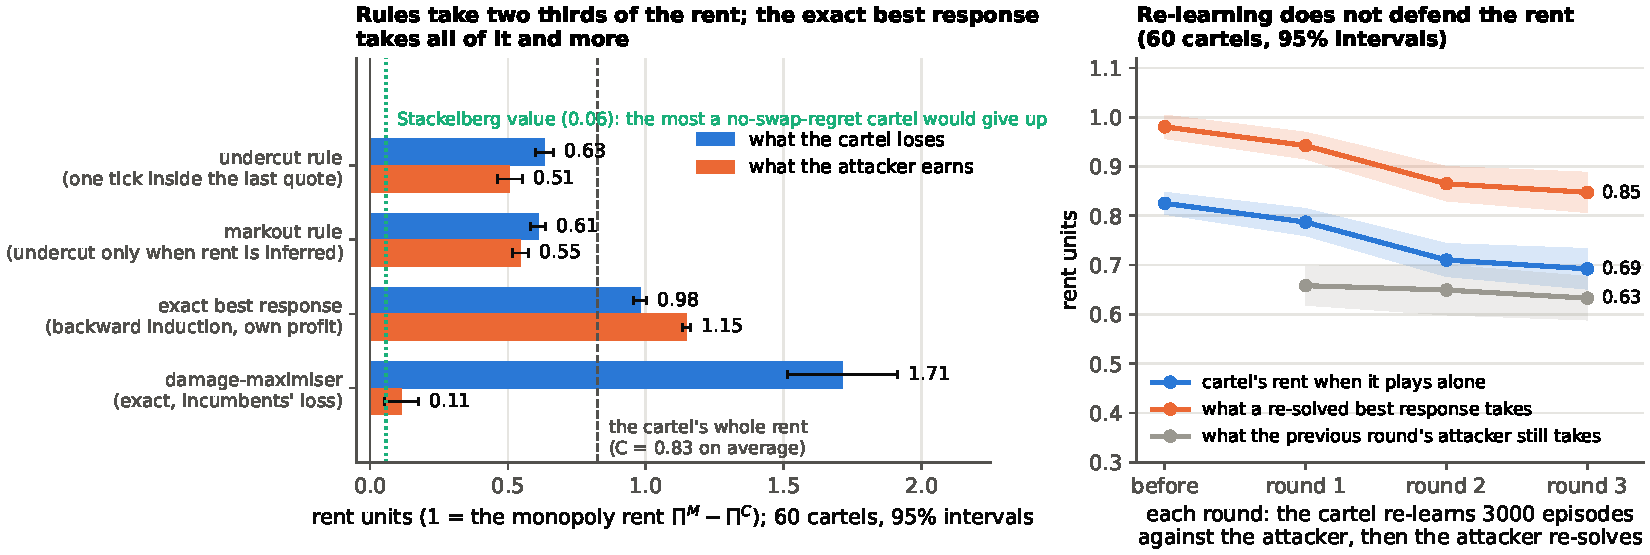
\includegraphics[width=0.9\textwidth]{fig_attackers.pdf}
\begin{itemize}\small\setlength\itemsep{1pt}
\item Rule adversaries destroy a flat $\kappa_A\approx0.7$ of the rent whatever $C$ (180 cartels). \textbf{The exact best response} --- backward induction over the frozen cartel's reaction function --- takes it all: $\LBR>C$ in 60/60 cartels, the entrant earns the monopoly profit, $\kappa_A=1.1$--$1.3$.
\item \textbf{How:} it undercuts the \emph{reaction}, not the last fill, and holds the cartel in states it never trained on, where its response is to quote \emph{wider}. The damage-maximiser steers it \emph{tight}, inside break-even: 2--3$\times$ the rent destroyed at zero cost.
\end{itemize}
\end{frame}

\begin{frame}{Evidence 3 --- what identity is worth, and why (RQ1)}
\centering
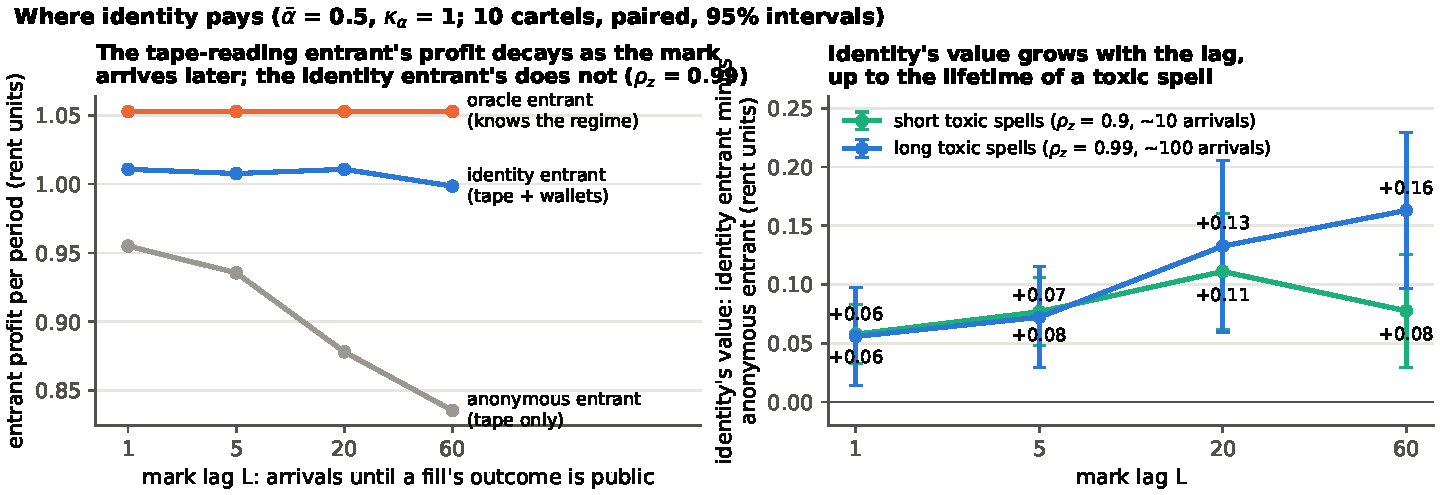
\includegraphics[width=0.88\textwidth]{fig_lag.pdf}
\begin{itemize}\small\setlength\itemsep{1pt}
\item The proposal's mechanism (the same wallet trades again) is worth nothing on the data: same-wallet repeats are 2--5\%.
\item The mechanism that survives: informed flow comes in \textbf{spells}; a wallet's fill reveals the spell \emph{before} the price does. Identity's value is zero where even the toxic state leaves an undercut profitable ($\bar\alpha\le0.3$), and grows with the mark lag up to the spell's lifetime.
\end{itemize}
\end{frame}

\begin{frame}{Evidence 4 --- Hyperliquid: the price cannot move, and someone still earns the spread}
\begin{columns}[T]
\begin{column}{0.55\textwidth}
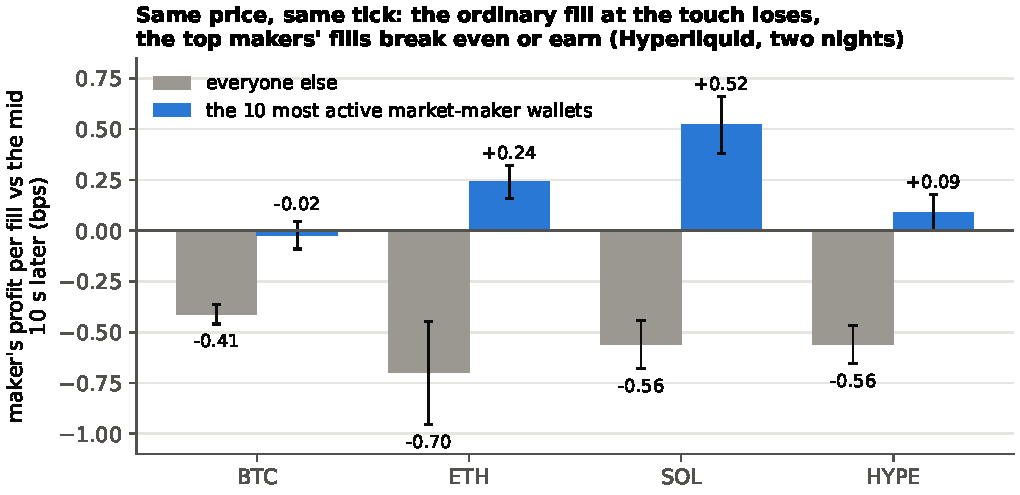
\includegraphics[width=\textwidth]{fig_touch.pdf}
\end{column}
\begin{column}{0.45\textwidth}\small
Two nights of best-bid/ask recording (15 h, 300k scored fills) $+$ 327 h of fills with both wallets.
\begin{itemize}\setlength\itemsep{2pt}
\item The quoted spread on BTC/ETH/SOL is \textbf{one tick essentially always} (p90 $=$ median). Rent cannot live in the price.
\item A fill at the touch pays that tick, then \textbf{loses 0.3--0.6\,bps} to the mid within 10 s, on every coin. The taker's cost is in depth: one order in ten walks the book and pays twenty ticks.
\item The ten most active maker wallets (chosen on activity, scored on outcome) earn \textbf{0.4--1.1\,bps more per fill at the same price}, and their ranking persists across nights (rank corr.\ 0.43--0.75).
\end{itemize}
\takeaway{Rent lives in \emph{which fills you get}, not in the quote.}
\end{column}
\end{columns}
\end{frame}

\begin{frame}{Evidence 5 --- how they do it: identity, not the tape}
\centering
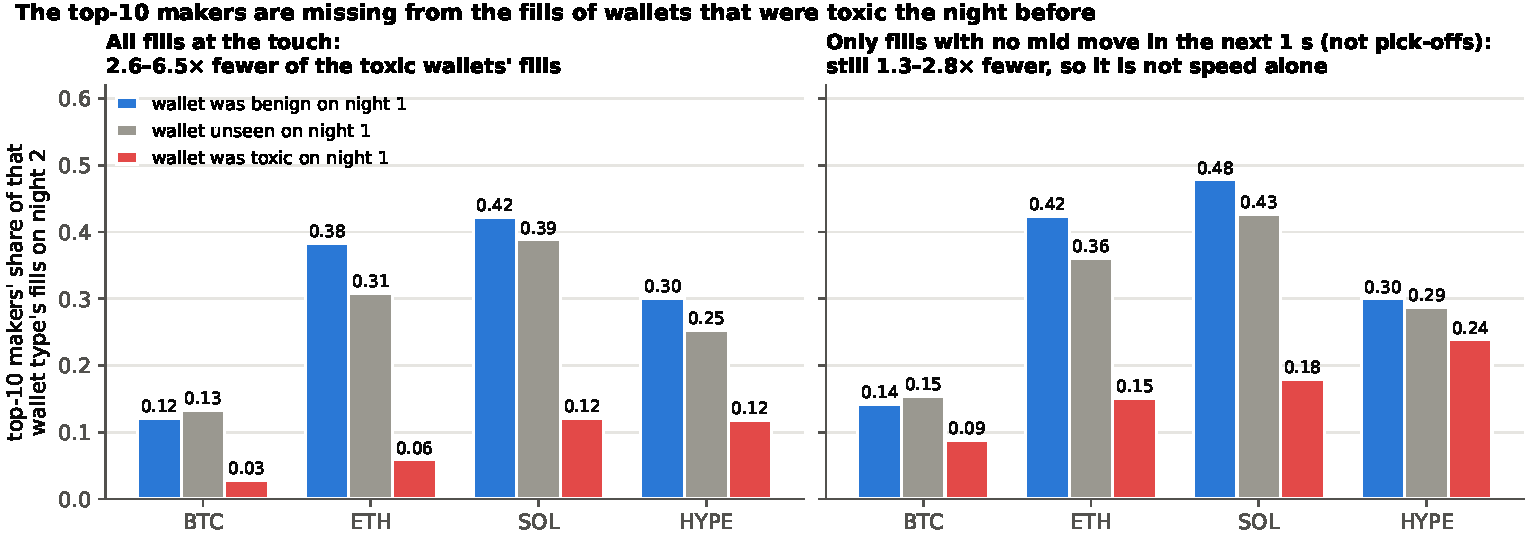
\includegraphics[width=0.86\textwidth]{fig_identity_selection.pdf}
\begin{itemize}\small\setlength\itemsep{1pt}
\item They never withdraw after a stressful spell at any timescale (30 s--5 min; correlations $-0.07$ to $+0.13$). They are absent from the \emph{wallet}, not the \emph{moment}: the gap is the same inside calm and stressed tape.
\item Classified on night 1, scored on night 2 (toxic wallets cost 1.0--2.3\,bps more on night 2: the typing holds). \textbf{RQ1's mechanism, observed on the real book.}
\end{itemize}
\end{frame}

\begin{frame}{Evidence 6 --- the levers decide who holds the toxic flow, not whether the rent survives (RQ3)}
\centering
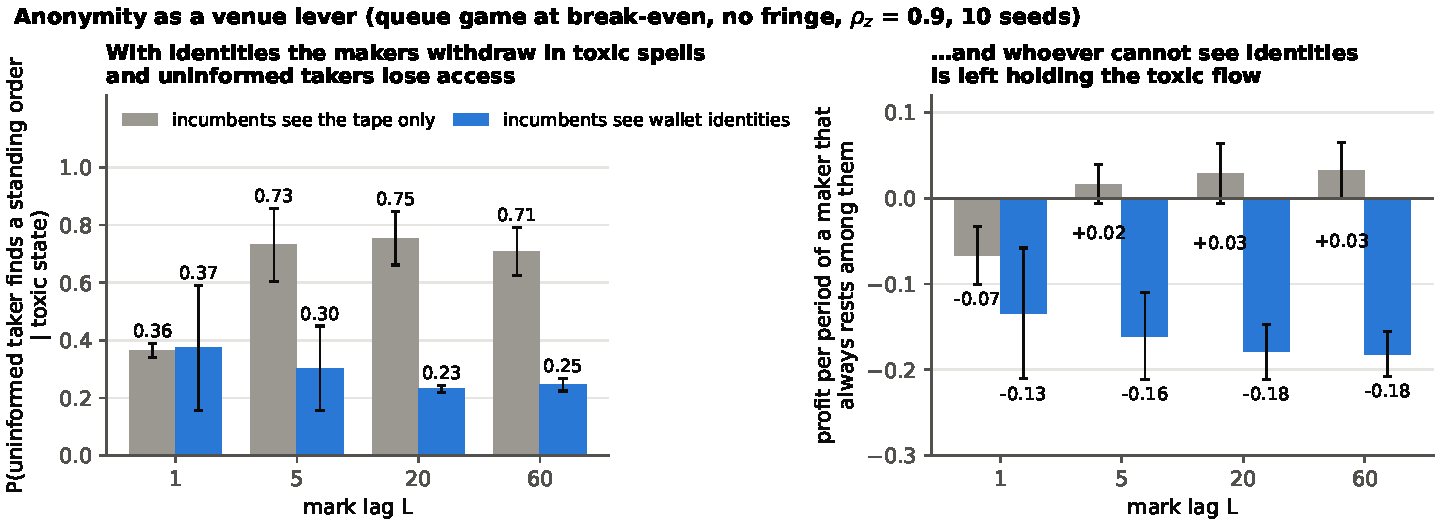
\includegraphics[width=0.74\textwidth]{fig_anonymity.pdf}
\begin{itemize}\small\setlength\itemsep{1pt}
\item \textbf{Anonymity} is a transfer from makers to uninformed takers in stress; \textbf{identity} the reverse. Neither defends the rent.
\item \textbf{Priority fee}: an all-pay auction for position; at the venue's optimum it collects 2--4$\times$ the makers' rent and leaves every maker at or below zero; the identity-blind fringe pays.
\item \textbf{Makers' own levers}: only the identity-aware floor improves both profit and resilience, only where the toxic regime bites, and it still leaves the adversary 75--80\% of its take.
\end{itemize}
\end{frame}

% ============================================================ (d) next steps
\section{Next steps}

\begin{frame}{Plan for Workshop 2}
\begin{columns}[T]
\begin{column}{0.5\textwidth}\small
\textbf{Attacks and learning}
\begin{enumerate}\setlength\itemsep{2pt}
\item \textbf{The attacker with public information only}: identify each incumbent's reaction function from the tape (every answer to (own, rival) is public; the entrant sets ``rival'' with its own quote), then solve. Report its gap to the exact best response vs the probing budget.
\item \textbf{Both sides learning}: PSRO with re-learning cartels and learned entrants --- the equilibrium's rent and $\kappa_A$; are adversarially trained cartels less exploitable, or just less collusive?
\item \textbf{Queue-mode attacks}: steering no-regret incumbents; draining the request budget.
\end{enumerate}
\end{column}
\begin{column}{0.5\textwidth}\small
\textbf{Resilient designs, and data}
\begin{itemize}\setlength\itemsep{2pt}
\item Venue levers (anonymity, tick, fee, request allowance) and maker levers on one frontier: (profit alone, profit in the worst 5\% of episodes under attack) against all three attackers, plus uninformed takers' access in stress --- so ``robust'' cannot mean ``withdrew''.
\item Weeks of recording (identity-selection gap by coin, hour, regime); the Oct 2025 liquidation cascade; the Dec 2025 order-level archive: \emph{which action} --- cancel, queue position, depth --- carries the selection.
\item Throughout: common random numbers, paired intervals, worst-5\% outcomes, train-at-$\bar\alpha$/test-at-$\bar\alpha'$, held-out adversaries.
\end{itemize}
\vspace{4pt}
\textbf{What we would value your view on:} is identifying a frozen reaction function the right ``realistic attacker'', or should the cartel be allowed to adapt continuously?
\end{column}
\end{columns}
\end{frame}

\appendix
\begin{frame}{Backup --- Hyperliquid numbers}
\scriptsize
\begin{tabular}{lcccc}
\toprule
 & BTC & ETH & SOL & HYPE \\
\midrule
one tick (bps) & 0.12 & 0.39 & 0.86 & 0.11 \\
taker's cost vs the mid: fills at the touch / walked (bps) & 0.12 / 2.35 & 0.42 / 3.20 & 0.92 / 5.20 & 0.17 / 3.57 \\
10-s maker markout, at the touch / walked (bps) & $-0.41$ / $-0.80$ & $-0.56$ / $-2.26$ & $-0.27$ / $+0.98$ & $-0.45$ / $-0.01$ \\
next fill's markout after a toxic vs a benign wallet (bps, 327 h) & $-0.64$ & $-1.01$ & $-0.59$ & $-0.59$ \\
10-s markout at the touch: top-10 makers / everyone else (bps) & $-0.02$ / $-0.41$ & $+0.24$ / $-0.70$ & $+0.52$ / $-0.56$ & $+0.09$ / $-0.56$ \\
per-maker rank correlation, night vs night ($n$ makers) & 0.75 (108) & 0.50 (65) & 0.56 (45) & 0.43 (68) \\
top-10 share of touch fills: benign / unseen / toxic wallets & .12 / .13 / .03 & .38 / .31 / .06 & .42 / .39 / .12 & .30 / .25 / .12 \\
\ldots\ on fills with no mid move in 1 s: benign / toxic & .14 / .09 & .42 / .15 & .48 / .18 & .30 / .24 \\
\bottomrule
\end{tabular}
\vspace{4pt}

Standard errors cluster by five-minute block; every top-10-vs-rest gap exceeds four SEs. Wallet types from night 1, scored on night 2.
\end{frame}

\begin{frame}{Backup --- the double oracle and robustness, in numbers}
\small
\begin{itemize}\setlength\itemsep{3pt}
\item \textbf{Double oracle} (cartel re-learns 3000 episodes against the fixed best response, entrant re-solves; 3 rounds): the now-stale attacker's profit falls $1.2\to0.5$ (the undercut-rule level); the re-solved one takes $\ge90\%$ of the remaining rent in every cartel every round; the cartel's own rent erodes $0.83\to0.79\to0.71\to0.69$.
\item \textbf{Damage-maximiser} ($\lambda=0$): steers the cartel to 4--7 ticks, inside break-even ($h^C=8$--$13$), by quoting above it; takes no fills, earns $\approx0$; $\LBR=1.3$ ($\bar\alpha=0.3$), $2.7$--$2.8$ ($\bar\alpha=0.5$).
\item \textbf{Train at $\bar\alpha$, test at $\bar\alpha'$}: cartels keep $C=0.80$--$0.86$, $\kappa_A=0.65$--$0.75$ (rules) on calmer markets; on a more toxic one the rent collapses ($C=0.23$) and is more than destroyed.
\item \textbf{Held-out adversaries} preserve every defence ordering (rank correlation $0.75$--$0.96$).
\item \textbf{Caveat we own:} the exact best response needs the cartel's reaction function (oracle knowledge of the \emph{policy}). It is the true upper bound; the public-information attacker that identifies it is next.
\end{itemize}
\end{frame}

\begin{frame}{Backup --- the queue game and the priority fee}
\small
\begin{itemize}\setlength\itemsep{3pt}
\item Learned incumbents need a \textbf{fringe} of always-resting makers (else a toxic spell empties the book for good); tabular Q cannot learn to queue (time priority pays only after consecutive periods in line); \textbf{no-regret (EXP3)} incumbents over complete policies learn to select in a few hundred episodes.
\item Against selecting incumbents identity is worth \emph{more}: $+0.05$ to $+0.06$ per period at every lag, 5/5 seeds; the fringe's payoff falls to $-0.02$ to $-0.10$ --- identity-blind resting liquidity is the counterparty of the selection rent.
\item \textbf{Priority fee}: every selector pays in calm periods (identity-aware incumbents 93--94\% of calm, 8--9\% of toxic periods); a non-paying entrant among payers gets 0\% of fills; the fringe's loss triples at any fee; revenue peaks at $f=0.5$.
\item \textbf{Makers' levers} (20 cartels, 7 adversaries incl.\ a Q-learning one): requoting every 2--5 periods costs everything; randomising costs profit and buys nothing; the identity floor: worst-case profit $0.08\to0.19$ at $\bar\alpha=0.5$.
\end{itemize}
\end{frame}

\end{document}
